%%% template.tex
%%%
%%% This LaTeX source document can be used as the basis for your technical
%%% paper or abstract. Intentionally stripped of annotation, the parameters
%%% and commands should be adjusted for your particular paper - title,
%%% author, article DOI, etc.
%%% The accompanying ``template.annotated.tex'' provides copious annotation
%%% for the commands and parameters found in the source document. (The code
%%% is identical in ``template.tex'' and ``template.annotated.tex.'')

\documentclass[]{acmsiggraph}
\usepackage{algorithm}
\usepackage[noend]{algpseudocode}
\TOGonlineid{45678}
\TOGvolume{0}
\TOGnumber{0}
\TOGarticleDOI{0}
\TOGprojectURL{}
\TOGvideoURL{}
\TOGdataURL{}
\TOGcodeURL{}
\usepackage{color}
%\definecolor{red}{rgb}{0.9, 0.17, 0.31}
\usepackage{multirow}
\usepackage{subfig}
\usepackage{xcolor}
\usepackage{lipsum}
\usepackage{listings}
\usepackage{graphicx}
\usepackage{glsllst} % My own package providing markup listing for glsl
\usepackage{rmlst}   % My own package providing markup listing for renderman
\usepackage{amsmath}
\usepackage{hyperref}

\lstset{
	backgroundcolor=\color[rgb]{0.95, 0.95, 0.95},
	tabsize=3,
	%rulecolor=,
	basicstyle=\footnotesize\ttfamily,
	upquote=true,
	aboveskip={1.5\baselineskip},
	columns=fixed,
	showstringspaces=false,
	extendedchars=true,
	breaklines=true,
	prebreak = \raisebox{0ex}[0ex][0ex]{\ensuremath{\hookleftarrow}},
	frame=none,
	aboveskip=15pt,
	belowskip=8pt,
	captionpos=t,
	showtabs=false,
	showspaces=false,
	showstringspaces=false,
	identifierstyle=\ttfamily,
	%keywordstyle=\color{red}\bfseries,
	%keywordstyle=[1]\bfseries\color{syntaxBlue},
	%keywordstyle=[2]\bfseries\color{syntaxRed},
	%keywordstyle=[3]\color{blue}\bfseries,
	%keywordstyle=[4]\bfseries\color{syntaxBlue},
	commentstyle=\color[rgb]{0.082,0.639,0.082},
	keywordstyle=[1]\bfseries\color[rgb]{0,0,0.75},
	keywordstyle=[2]\bfseries\color[rgb]{0.5,0.0,0.0},
	keywordstyle=[3]\bfseries\color[rgb]{0.127,0.427,0.514},
	keywordstyle=[4]\bfseries\color[rgb]{0.4,0.4,0.4},
	stringstyle=\color[rgb]{0.639,0.082,0.082},
}

\title{Simulation Techniques for Animation: GPU Accelerated Mass Spring System}

\author{Joe Withers\thanks{e-mail:joewithers96gmail.com}}
\pdfauthor{Joe Withers}

\keywords{simulations}

\begin{document}

%% \teaser{
%%   \includegraphics[height=1.5in]{images/sampleteaser}
%%   \caption{Spring Training 2009, Peoria, AZ.}
%% }

\maketitle


\begin{abstract}
This document serves to demonstrate the short paper format used for the Principles of Rendering unit. This submission should be no longer than 2 pages, inclusive of references and images, but excluding appendices and code listings. You should aim for between 5 and 8 references in your bibliography.
An abstract provides an executive summary of your short paper.
\end{abstract}
%\keywordlist
%\TOGlinkslist

\section{Introduction} \label{sec:introduction}
In this section you should introduce the shader effect you're trying to recreate. You should include a few examples of real reference images which you are trying to simulate, such as in Figure~\ref{fig:reference}. You must also decompose the chosen effect into individual layers or effects which you are going to try to implement.

\begin{figure}[htbp]\centering
 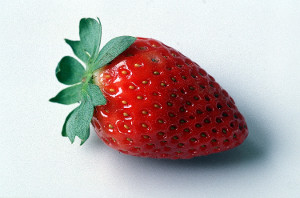
\includegraphics[width=0.75\linewidth]{images/strawberry.jpg}
 \caption{\label{fig:reference}An example reference image, acquired from \protect\cite{fruits16}.}
\end{figure}

For example, the strawberry in Figure~\ref{fig:reference} might exhibit:
\begin{enumerate}
 \item Regular seed placement which causes small indentations in the surface.
 \item A gentle colour gradiation from tip to top.
 \item Narrow specular highlights.
 \item Shallow subsurface scattering properties.
 \item Soft shadowing.
 \item Slight depth of field effect.
\end{enumerate}
You might also use this section to introduce examples of how this effect may have been created in the past, particularly in books, industry talks or academic papers, where the method used to recreate the effect is known. Make sure you make use of references here, such as \cite{rtr08} or \cite{pbr10} in order to contextualise your work.

\section{Method Overview} \label{sec:overview}
In this section you should present the final method which you have implemented in a manner that is as independent of the language used to create the effect as possible. There are a number of different ways to do this, for example using a mathematical formulation as in Equation~\ref{eq:kajiya}.
\begin{multline}\label{eq:kajiya}
L_o \left( \mathbf{x},\omega_o,\lambda,t \right) = L_e\left(\mathbf{x},\omega_o,\lambda,t \right) + \\
   \int_\Omega f_r \left(\mathbf{x},\omega_i,\omega_o,\lambda,t\right) L_i\left(\mathbf{x},\omega_i,\lambda,t\right) \left(\omega_i \cdot \mathbf{n}\right) d\omega_i
\end{multline}
Alternatively you might want to present your method in the form of a pseudocode algorithm, as in Algorithm~\ref{alg:euclid}.
\begin{algorithm}
\caption{Euclid’s algorithm}\label{alg:euclid}
\begin{algorithmic}[1]
\Procedure{Euclid}{$a,b$}\Comment{The g.c.d. of a and b}
\State $r\gets a\bmod b$
\While{$r\not=0$}\Comment{We have the answer if r is 0}
\State $a\gets b$
\State $b\gets r$
\State $r\gets a\bmod b$
\EndWhile\label{euclidendwhile}
\State \textbf{return} $b$\Comment{The gcd is b}
\EndProcedure
\end{algorithmic}
\end{algorithm}
You will probably also find that data flow diagrams\footnote{See \url{https://en.wikipedia.org/wiki/Data_flow_diagram}.} are very useful in conveying how your shader is implemented using OpenGL when multiple render passes are needed.

You should avoid describing your method using code examples if possible. If you must, an example of code inclusion and markup is provided in Appendices~\ref{app:renderman} and~\ref{app:glsl}.

\section{Results} \label{sec:results}
Here you should present the rendering results of the method(s) which you have described in Section~\ref{sec:overview} above. Ideally, you should provide a breakdown of the different layers or render passes used in the construction of the final effect (see Figure~\ref{fig:comparison} for an example). Where the geometry is complex, it might also be suitable to render a simple object (a sphere perhaps) to demonstrate the effect of the different render layers. If you are demonstrating a dynamic effect, you might want to render several frames of a sequence.

\begin{figure}[htbp]
  \centering
 \subfloat[Diff+Spec]{
\includegraphics[width=0.45\linewidth]{images/image1.jpg}}
 \hfill
 \subfloat[Diff+Spec+Ambient]{
\includegraphics[width=0.45\linewidth]{images/image2.jpg}}
 \caption{\label{fig:comparison}A side by side comparison of different render effects is always a good idea to demonstrate a choice of parameters or design of your shader. These were appropriated from \protect\cite{renderman16}.}
\end{figure}

If you are generating a real time effect, it might also be suitable to demonstrate with some numbers or statistics the performance improvements that you were able to attain by optimisations to your shader or C++ application.

You may also want to provide a discussion of development iterations and the thought processes by which you arrived at the final method presented in Section~\ref{sec:overview}. It is important in this section to be self-reflective and critical: we don't expect you to have created the perfect effect. If you are disatisfied by any aspect of the result, you should communicate this to us with some sort of explanation.

\bibliographystyle{acmsiggraph}
\bibliography{references}

\newpage
\appendix
\section{Renderman Shader Example}\label{app:renderman}
An example of Renderman code listing is included below. Please make sure that when including code segments that you include only sections that are directly relevant to the application at hand, and preferably which link to the method described in Section~\ref{sec:overview}.
\begin{lstlisting}[language=rendermansl, label={lst:renderman}, caption={Renderman example lifted from \protect\cite{renderman16}.}]
surface basicSpecular(
    color myOpacity = 1;
    float roughness = 0.1;
)
{
        color myColor = (1.0, 0.0, 0.0);
        normal Nn = normalize(N);
        //Specular stuff
        vector V = normalize(-I);

        Ci = myColor * myOpacity * diffuse(Nn) + specular(Nn, V, roughness);
        Oi = myOpacity;
}
\end{lstlisting}


\section{GLSL Shader Example}\label{app:glsl}
An example of a GLSL code listing is included below. Note that C++ code listing is also supported using the same method.

\begin{lstlisting}[language=GLSL, label={lst:glsl}, caption={A simple textured shader.}]
// The texture coordinates
smooth in vec2 o_TexCoord;

// This is passed on from the vertex shader
in vec3 LightIntensity;

// The texture to be mapped
uniform sampler2D u_Texture;

// This is no longer a built-in variable
out vec4 o_FragColor;

void main() {
    // Set the output color of our current pixel
    o_FragColor = vec4(LightIntensity,1.0) * texture(u_Texture, o_TexCoord);
}
\end{lstlisting}


\end{document}

